\documentclass[letterpaper, 12 pt, conference]{ieeeconf}
\IEEEoverridecommandlockouts
\overrideIEEEmargins
\usepackage{cite}
\usepackage{algorithm}
\usepackage{algpseudocode}
\usepackage{amsmath}
\usepackage{amssymb}
\usepackage{graphics}
\usepackage{graphicx}
\usepackage{wrapfig}
\usepackage{multirow}
\usepackage{rotating}
\usepackage{verbatim}
\usepackage[caption=false,font=footnotesize,subrefformat=parens,labelformat=parens]{subfig}
\usepackage{listings}
\usepackage{color}
\definecolor{dkgreen}{rgb}{0,0.4,0}
\definecolor{gray}{rgb}{0.5,0.5,0.5}
\definecolor{mauve}{rgb}{0.58,0,0.82}
\graphicspath{{graphics/}}
\DeclareGraphicsExtensions{.png}
\lstset{frame=tb,
  language=Python,
  aboveskip=3mm,
  belowskip=3mm,
  showstringspaces=false,
  columns=flexible,
  basicstyle={\small\ttfamily},
  keywordstyle=\color{blue},
  commentstyle=\color{dkgreen},
  stringstyle=\color{mauve},
  breaklines=true,
  breakatwhitespace=true,
  frame = L,
  tabsize=4
}
\title{\bf
Air-Hockey Robot
}

\author{\parbox{5 in}{\centering Daniel Koniar, Matthew Russell, and Steve Thomas}\\
  {\tt\small \{konia013, russe546, thom5159\}@umn.edu}\\
  Department of Computer Science and Engineering\\
  University of Minnesota\\
  Minneapolis, MN 55455\\
}  

\begin{document}
\maketitle
\thispagestyle{empty}
\pagestyle{empty}

%%%%%%%%%%%%%%%%%%%%%%%%%%%%%%%%%%%%%%%%%%%%%%%%%%%%%%%%%%%%%%%%%%%%%%%%%%%%%%%%
\begin{abstract}
This paper evaluates, and attempts to employ, the construction of a Air-Hockey Playing Robotic System in a real-time physical environment.  This project aims to increase understanding of the design, construction, and control of a robotic manipulator through a fast-paced environment utilizing new technology available for the design and implementation of robotics, including real time video capture and analysis and controlling motors through a microcontroller. We examine issues that crop up when undertaking such a task and what methods worked well.
\end{abstract}

\section{Introduction}
\label{introduction}
Improvement in both robotic manipulators and computer vision has allowed for the production of complex robotic systems that are capable of reacting to a real-time environment. A variety of specialized robotics, varying from robotic drones \cite{3dr} with ground recognition to self-driving cars \cite{googlecar}, have been constructed using combinations of these components.  

This project combines computer vision and robotic mechanisms in an attempt to design and construct a complex robotic system capable of playing Air Hockey. In this project, multiple aspects will be examined and discussed.  One aspect will be the analysis of the actual design and construction of the Air Hockey robot.  As each component becomes functional, the results will be gathered and examined, the metrics may not be conventional. The last aspect of the project that will be examined is the entirety of project in a retrospective lens.  The analysis of this will include what could be done to make the system better and what failures were experienced.

There are many key metrics for the Air-Hockey Robot an order to attempt to reach an optimal state. The metrics that will be mainly emphasized are efficiency, reactionary time, accuracy, and repeatability. To further define these, efficiency will be defined as minimizing the movements necessary to be made by the robotic manipulator an order to hit the puck.  Reactionary time will be defined as the amount of time needed to go from raw images to movement input to the robotic manipulator. Accuracy will be defined as how often the puck can be reached and hit in the desired direction [with a small error tolerance].  Repeatability will be defined as the robotic manipulator’s ability to repeat an action precisely, provided the exact same environment/situation. For instance, if a puck were sent from the same exact direction and with the exact velocity one hundred times, repeatability would be the number instances where the robotic manipulator could hit the puck in the same exact way.

To conclude the introduction, an overview of the outline of this paper is provided. This paper will first discuss the problem that is going to addressed. This section will further define the problem of designing and constructing an air hockey robot, the motivation to solve this problem, and related work that has been done on this topic. This section aims to first inform on the topic being addressed in this paper.

After that, this paper will further define and discuss the design of the air hockey robot. The design will be broken up into three sections, which are the robotic manipulator, the computer vision, and lastly the robotic system in total. Each will discuss the design options chosen and the design components that changed. 

The results section follows the design. This section simply reports the discoveries while building each component of the robotic system, as well as the robotic system in totale. It covers the initial design robotic manipulator design involving four servo motors, to the transition to two direct current motors and two stepper motors. 

The analysis section follows the results. While the design only discussed design decisions, the results section informs of the issues that were encountered forcing many of the design changes that were made. The analysis of the issues experienced that forced design changes are key to formulating a conclusion. The analysis looks at why certain design challenges were faced and how it led to the failure to construct an air hockey robot system in total, on a component to system level.

The last two sections are the conclusion and future work, respectively. The conclusion covers bringing all the key information together as a shorter compilation of the paper. This section is not split into subsections as it investigates the design and failures in total with information from all sections. The future work section addresses how research could be continued on this project and, if given more time, how success for constructing this robot could be achieved.

\section{Problem Description}
\label{problemdescription}
\subsection{Definition}
\label{definition}
Air Hockey is a two-player game where the players hit a puck across a table using mallets. The table used to play air hockey has elevated borders to prevent the puck from exiting the play field.  The table also has holes in the surface in a consistent, even pattern all across the board through, which air is passed through in order to elevate the puck and mallets, reducing friction. The goal of air hockey is to hit the puck into the other player’s goal. When the puck enters a player’s goal, the opposing player receives a point.  The first player to reach a predetermined score, or has the highest score after a set amount of time, wins the air hockey game.

A complex robotic system capable of playing air hockey will be designed through the combination of computer vision and robotic device manipulation.  This design will then be constructed, or rather attempted to be.  The goal of the air-hockey robotic system will be to protect its goal while attempting to defeat the opponent player.

Monolithic-structured software typically acts as the cohesive layering between the robotic and computer vision layers.  This software allows for a translation to be made from the input from one hardware component to output for another hardware component.  This allows for the robotic system to work intelligently in its workspace. 

Through this, it also allows for a goal or task to be defined within the robotic system.  Through translation of the input utilizing computer vision, it allows for response from the robotic mechanism in reaction to a changing environment through computational analysis.  One example of a robotic build with the same concept would be automated assembly systems, where computer-vision object-recognition is used in order to achieve the goal of a robotic manipulator grasping and transporting objects.

By combining computer vision and robotic mechanisms with a cohesive layer of software, an air hockey playing robot can be implemented with a goal-oriented approach to allow the robotic system to react to a human opponent’s actions and quickly derive a solution. The setup will require an overhead camera which monitors the puck movement and a robotic manipulator with the end effector being the mallet. The manipulator constructed onto the workspace, being the air hockey table, and was interfaced through a computing device.

The camera will track the puck movement in a two dimensional plane and the data will be processed through the computer vision software to compute the trajectory of the puck.  The trajectory will then be used by the mediary software to predict the movements for the robotic manipulator an order to strike the puck back towards the opposite goal [from which the robotic manipulator is defending].  The cohesive software layer will handle the transition of data from the computer vision software to the robotic manipulator, which will compute how the manipulator should react. The mallet will thus be controlled through a combination of robotic mechanisms and artificial intelligence in a reactionary setting.

\subsection{Motivation}
\label{motivation}
The primary motivation of this project is to increase understanding of real-time employments of computer vision in combination with robotic devices. Computer vision is widely used today with its applications ranging from traffic control\cite{aliane} to gesture recognition \cite{bhame}.  More specifically, computer vision is a tool used in robotics to capture and parse images to achieve a predefined goal. The robotic system takes in this image data and performs selective tasks based on the output from the image processing algorithms and functions written within the system. 

The secondary motivation is to experiment with the design and implementation of the software interface that combines two different hardware components. This design of many systems relies on well-defined planning and accommodation for change. This project will increase the understanding of the complexity of systems engineering.

The third motivation is to increase understanding about the significance of robotic accuracy and repeatability. Since the game of air hockey is a fast -paced environment, the robotic system response necessitates a fast reaction time.  This implies that the system’s hardware needs to be precise given proper input.  It also implies that the software needs to properly translate data from images to movement, while account for error.

\subsection{Related Work}
\label{relatedwork}
There has been numerous amounts of research in the design, construction, and control of a complex robotic system capable of playing air hockey in a real-time environment. The designs for this system vary across multiple components and factors.

One approach to the design was to use a robotic arm that had four degrees of freedom for mallet manipulation.  The base of the robotic arm was set just outside of the air hockey playfield while the end-effector grasped the mallet.  This system employed two cameras for puck tracking \cite{namiki}. Another approach had a simplified design compared to that previously mentioned. This approach varied by using a three degrees of freedom robotic arm and only one camera for puck detection \cite{bishop}. The designs from the approaches mentioned avoided complete integration with the air hockey table.

There has also been research done in the calibration of an air hockey robot. A group in Iran have a system to automatically calibrate the table’s intrinsic parameters for different table setups \cite{alizadeh}.  Additionally, work has been done to consider the interaction between a puck and the paddle hitting it, and what such forces mean for the motion of the puck \cite{ghazvini} \cite{iguchi}. Another group has researched predicting where the puck will be over time and fuzzy logic control involved in this methodology \cite{wang}.

Feature matching is an important part of image processing and could be used to track the puck and possibly the robotic manipulator position and velocity. Since motion requires more than one frame, velocity will be determined through the comparison of two image feature matches \cite{rahman}. Two algorithms that could be attempted for puck detection and tracking are SIFT feature matching and thresholded contour detection. SIFT will likely give more accurate results, however SIFT feature matching can be too slow given a real-time environment. There are alternatives to SIFT feature matching, which involves thresholding and trying to match shapes \cite{wang} \cite{marra} \cite{bishop}. The SIFT feature was decidedly the initial route to take for implementation, but the fallback will either thresholding and shape matching.

\section{Design}
\label{design}
\subsection{Robotic Manipulator}
\label{design-roboticmanipulator}

\begin{figure}[!h]
\centering
\subfloat{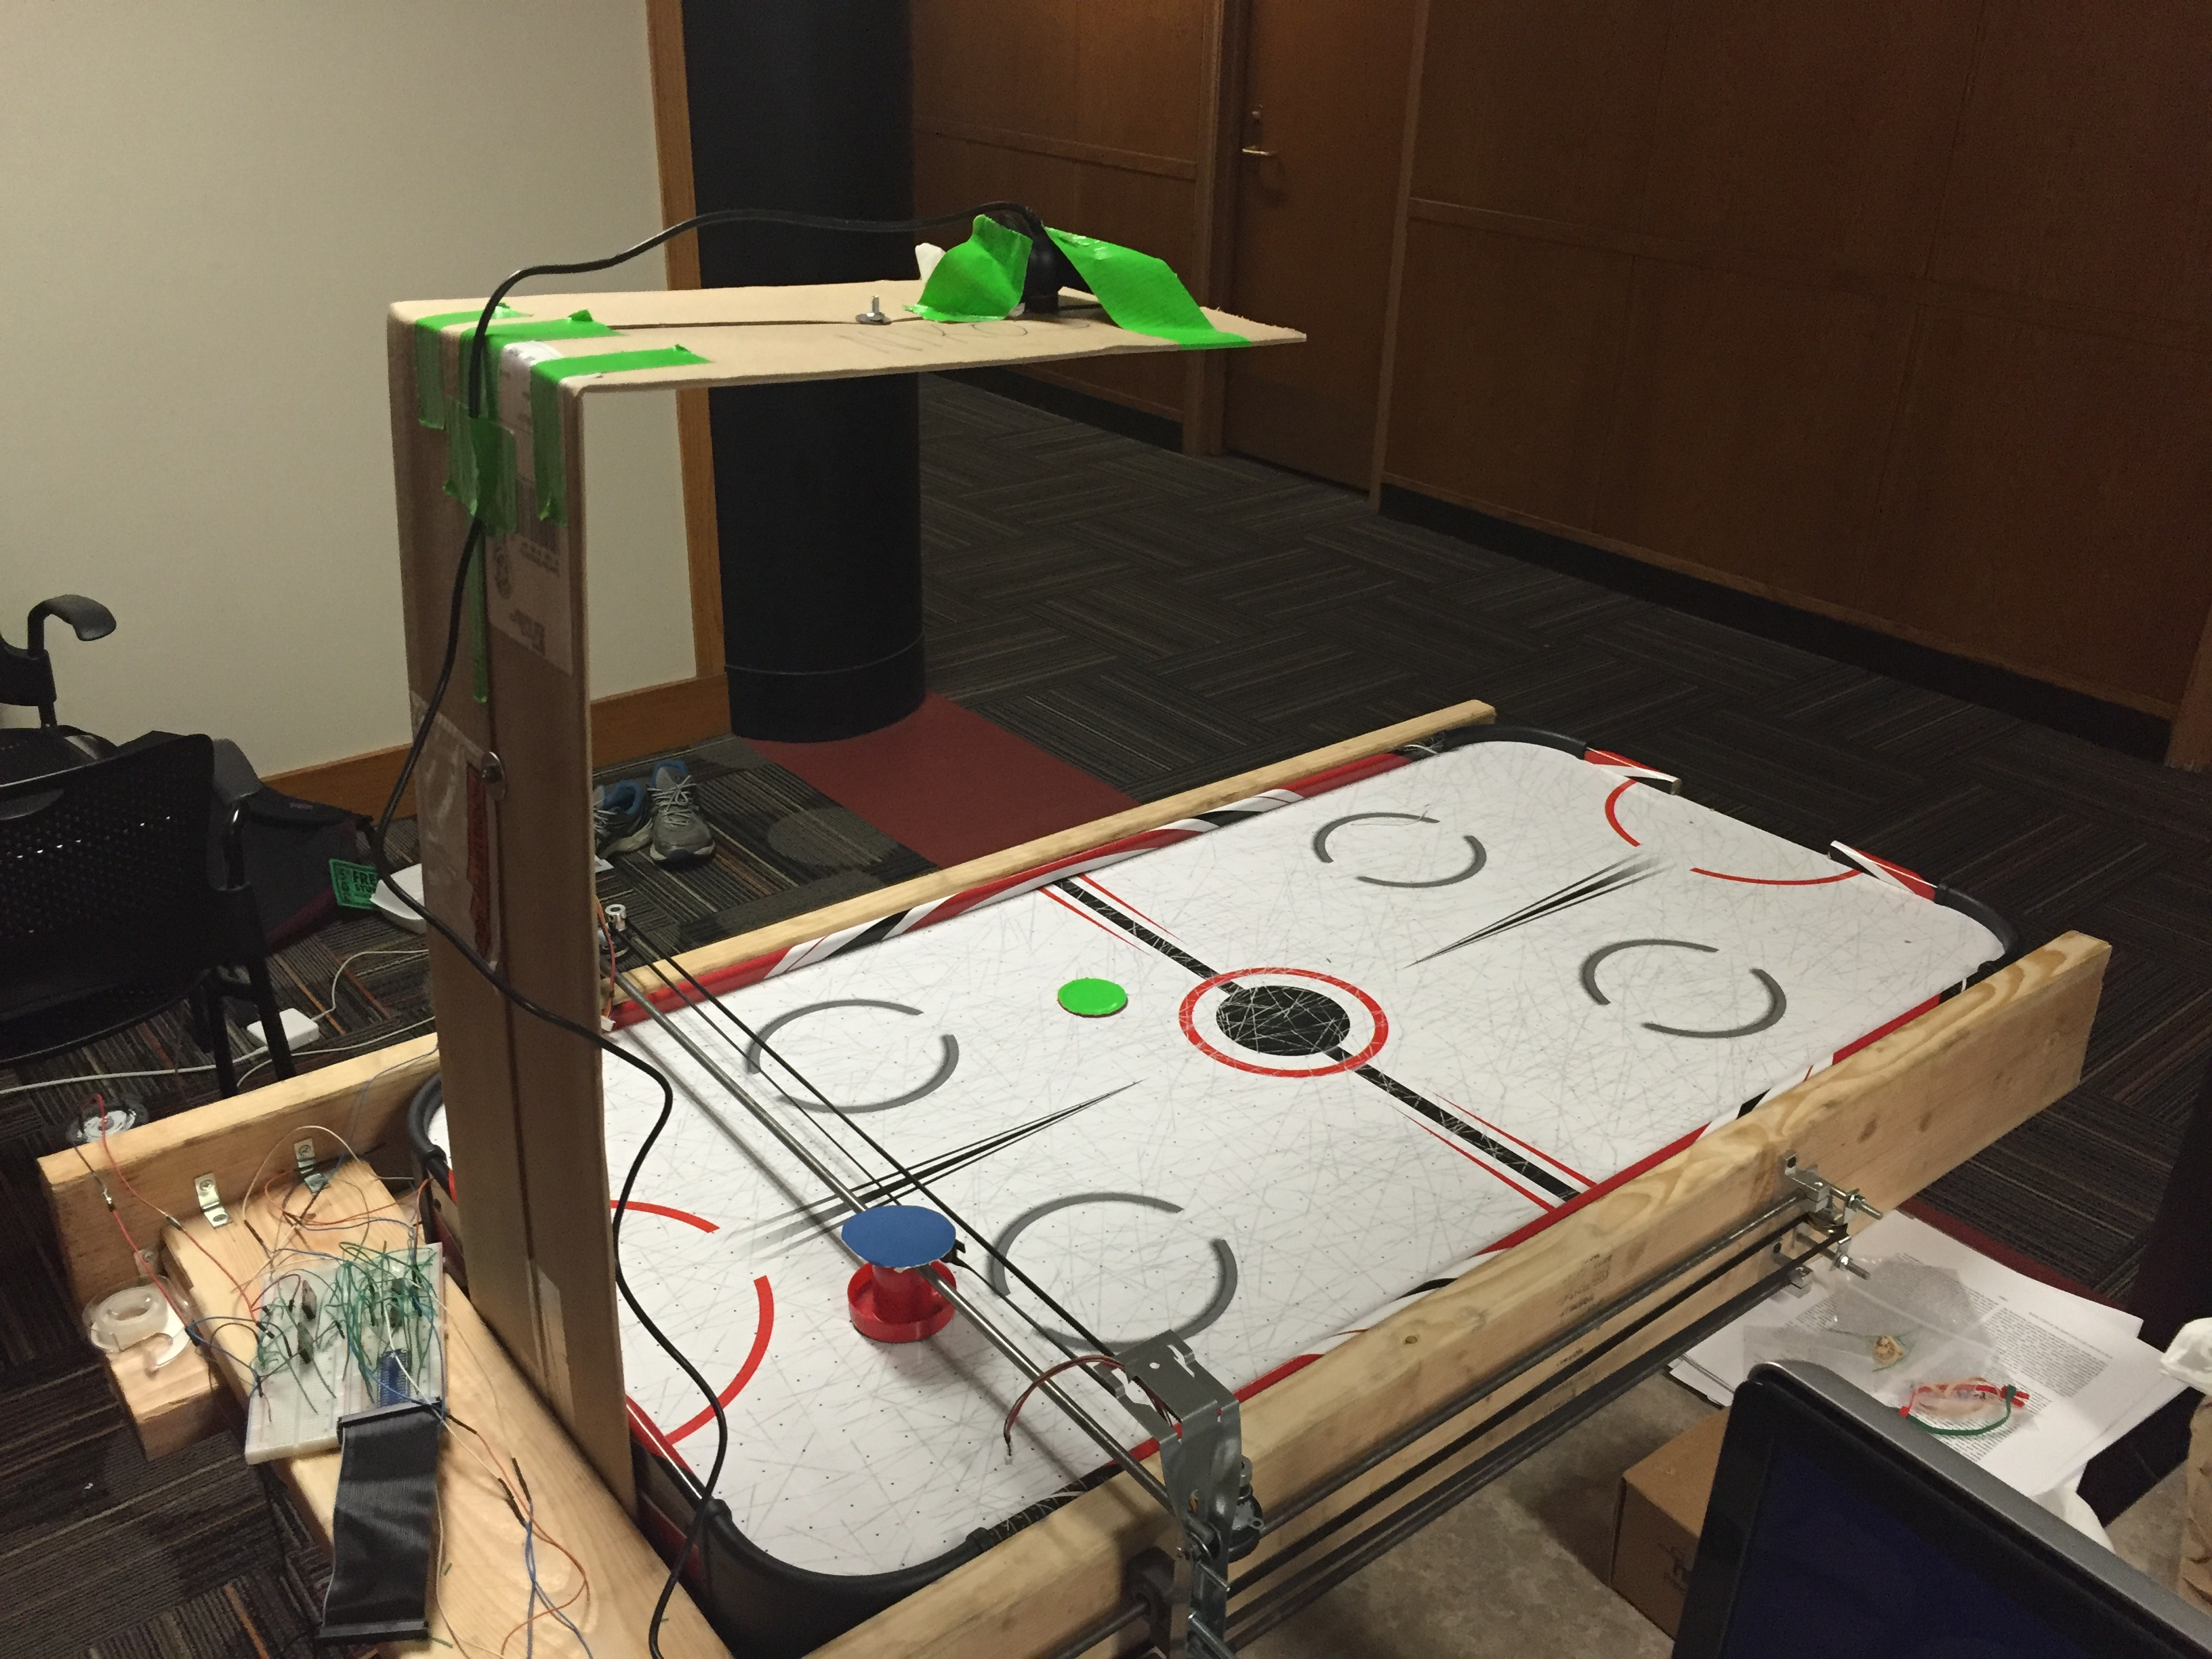
\includegraphics[height=8.5cm, width=8.5cm]{airhockeysystem}%
\label{airhockeysystem}}
\caption{The Air Hockey Robot}
\end{figure}

The robotic manipulator of the air hockey robot is designed to enable movement in two dimensions of motion. This is due to the fact the entire gameplay of an air hockey system is limited to one plane. Therefore, the manipulator for such a system would need inhibited motion on the plane while playing against a player.

The objective of the robotic manipulator is to control the end effector, which in this case is the mallet or striker. This could have been done through number of ways. For one, the use of robotic arm could do job. However, the use of multi-link robotic manipulator could turn inefficient as the control of the such a manipulator would be too complex for such a system. Due to the fast paced nature of the game, it is essential to get rid of any redundancies which could possibly slow down the response time of the system.

Hence, the preferred choice for design of such a system would have to be a two degree of freedom prismatic manipulator. The basic a design consists of mounting the motors on the edges of the workspace to system. The motors are used to drive belts wrapped around them. One set of belts runs along the edges of the air hockey table parallel to each other. These belts control the motion along one direction of the board. Attached onto these belts is the second belt whose length is perpendicular to the them. Attached to its own set of motors, the functionality of the second belt is to control the motion along the second direction of motion. On this belt we attach the mallet, which is the end effector used to play against the player.

The advantage of such a setup enabled for a simpler design, which could execute faster in real time and avoid any complexities. These avoided complexities would have occurred with a more sophisticated robotic manipulator. This is a key motivation when dealing with a complex robotic system as the game of air hockey demands high speed response from the robotic manipulator.

Besides the design of the robotic manipulator, it is important to select the right hardware needed to build manipulator. For motors the choice varied from steppers, servos, and DC motors. In the end, the choice of two steppers and two DC’s was used. The steppers used were the 5VDC 32-Step 1/16 Gearing reduction stepper, which provides a 80 rpm at 12 volts input. The second pair of motors were 12VDC motors. These motors provide great torque at high input voltages. 

The motivation of using steppers was the same as that with servos. In both motors, the rotations were quantified based on the number of steps or degrees. This provides a higher level of precision in terms of positioning the mallet along the x-axis of the board. The prismatic joints along the y-axis of the board were DC motors. Since DC motors are harder to control and quantify in terms of steps, they were used solely for their speed capabilities. This means that the DC motors would provide a fast impulse when switched on momentarily so the mallet could be pushed to hit the puck when it came close.

The integrated circuits used were the motor driver circuits L293D and the L298N. A total of three integrated circuits were used. Two L293D were used to control the two steppers each and one L298N used drive the pair of DC motors. The L293D and L298N are H-bridges used to interface the motors with a controller. The input voltages applied to the two steppers were 15 volt DC each and 12 volt Dc to Dc motors together. 

Specialized materials were ordered to to develop the design mechanisms. Belt pulleys and timing belts were used. The belt pulleys were mounted on the motor rotors and timing belts were used. Timing belts have teeth to protect from slipping and over the pulleys. Along with that, linear rails were ordered to provide support to the belts and the guides for the shuttles to which the steppers were mounted. The shuttles were mounted on the linear rails on specialized linear bearings.

\subsection{Computer Vision}
\label{design-computervision}
To facilitate input to the robot, a web camera was utilized as a cheap and easy source of information. The PS3EYE webcam suited this purpose since it was a cheap component and the Raspberry Pi, the computing device for the robotic system, had drivers for it pre-installed. The computer vision library openCV3 \cite{opencv} introduced a simple function to grab frames from this camera. 

The puck and striker were marked using primary and secondary colors. In this case, bright green and blue were used as these colors are easy to threshold from colors already present in the background of the air hockey table, which contained primarily reds, blacks, and white colors. The image taken from the webcam is reduced in size by a factor of four to improve run-time, as the objects the algorithm needs to detect are quite large compared to the background noise. Since the objects are in a fixed plane relative to the camera, the relative size of the image does not matter as long as there is enough resolution to adequately see the colors required. 

To further reduce noise, a Gaussian blur was applied to the resized image. The image is then converted to HSV to make the thresholding easier, and masked for each color that is needed, using predefined thresholds. These masked images are then passed to OpenCV’s findContours function \cite{opencv}. The algorithm then finds the largest of the contours above a certain threshold, and computes its centroid.

Because the findContours function returns all possible contours, there is still a lot of noise in the form of tiny contours. This data is filtered to only return the largest contour above a defined cutoff size. If the size of the contour is sufficiently small, the algorithm can be reasonably confident that the object is not yet in view. In the Figures \ref{frame_0}, \ref{frame_1}, and \ref{frame_2}, the puck is colored red and the striker is colored blue, a green dot shows what objects are being tracked by the algorithm.

\begin{figure*}
\centering
\subfloat{\includegraphics[height=6cm, width=12cm]{frame_0}%
\label{frame_0}}
\caption{Only the blue striker is located as the red puck is not far enough in frame to register}
\end{figure*}


\begin{figure*}
\centering
\subfloat{\includegraphics[height=6cm, width=12cm]{frame_1}%
\label{frame_1}}
\caption{The puck comes into view and the algorithm begins to track it.}
\end{figure*}



\begin{figure*}
\centering
\includegraphics[height=6cm, width=12cm]{frame_2}%
\label{frame_2}
\caption{The puck’s position has been found twice, and as such the puck’s direction and speed can be calculated}
\end{figure*}


The algorithm stores the positions it has previously tracked and, when it has discovered the striker’s position and the puck’s position twice consecutively, it has enough information to plan future trajectories and determine an intercept path for the striker. This future point of contact is determined using the following equation:
\begin{equation}
(P_{x} + {{P v_{x} * (S_{y} - P_{y})}\over{P v_{y}}}, S_{y})
\end{equation}
to find the $(x, y)$ coordinate where the puck will cross the striker’s x-axis, where $P$ is the position of the puck at this timeframe, $Pv$ is the speed of the puck at this time frame, and $S$ is the striker position at this time frame. 



\begin{figure}[!h]
\centering
\subfloat{\includegraphics[height=8cm, width=8cm]{trajectory}%
\label{trajectory}}
\caption{Determining where the puck will cross the striker’s x-axis}
\end{figure}


\subsection{Robotic System}
\label{design-roboticsystem}
The robotic system can be divided into three main parts. This division is based on how the air hockey robot takes in inputs, processes and responds to the given input, and the generated output. The robotic system was designed with both the robotic manipulator (see section \ref{design-roboticmanipulator}) and the computer vision (see section \ref{design-computervision}) components integrated with a cohesive layer of software. The abstraction of this design is presented in a monolithic structure, which can be seen in Figure \ref{systemdiagram}.  

The cohesive software layer that combines the computer vision and robotic manipulator components of this project handles input and translate it to output for the manipulator, which can be seen diagrammed in Figure \ref{systemdiagram}.  It would handle communication with the robotic manipulator software and the computer vision software as well as maintaining state data for the system.  This component would integrate the two major components of the project into a single complex system that would be capable of accomplishing a specialized task.

\begin{figure}[!h]
\centering
\subfloat{\includegraphics[height=7cm, width=7cm]{systemdiagram}%
\label{systemdiagram}}
\caption{Monolithic structure of the Air Hockey Robot}
\end{figure}

The Air Hockey playing robot takes in data from the camera mounted on the system. This camera tracks the positions of the puck and mallet simultaneously. The camera captures these position coordinates by grabbing frames from the camera.
These frames are then fed to the Raspberry Pi which processed the information, through the cohesive software layer mentioned previously.

On the processing side, the data is fed into the system. This data is filtered and then processed to pinpoint the exact position of the puck and end effector on the workspace. Based on these positions, the robotic system determines how the mallet, or end effector, should move based on its own position and that of the puck.  Multiple positions can then be used to compute the speed of the puck and the maximum speed the mallet can travel. Since the puck and mallet should have a constant velocity, these equations should be linear in nature.

Furthermore, the robotic system would be integrated into the air hockey table. By going with an integrated design, the component of calibration could be lessened. Since there wouldn’t be a necessity to align the robot each time in a three dimensional plane or rather x, y, and z relative to the table position. This was the main reason the design incorporated an integrated design despite numerous works using a detached robotic component (See Section \ref{relatedwork}).

\section{Results}
\label{results}
\subsection{Mallet Manipulation}
\label{results-malletmanipulation}
The mallet manipulation was done by a specially-designed manipulator which consisted of prismatic joints whose motion were perpendicular to each other. The idea was to construct a simple two degree of freedom robotic manipulator which performed efficiently and had a quick response time. However, although the design was estimated to work really well, some problems were encountered during the construction and testing phase of the system. 

From the start, the design of the robotic manipulator involved servo motors. However, due to the structure of the the servo body design, an issue with mounting the servos on the system was encountered. Also, the servos were meant for high torque applications, which resulted in a low rotational speed. Therefore the motors were switched to a combination of DC motors (for speed) and stepper motors (for precision). The steppers were interfaced to the L293D each and the were driven to a voltage of 15 volts at 1 A each.

However, on close observation it was noticed that the motors were underpowered and caused the end effector to move at a slow rate along the x-axis. On trying to provide more power to the motors, the integrated circuits (IC) were burnt, despite the fact that the power provided were well within the specified range of the IC capacity. Hence, there seemed no way to provide more power to the steppers.

The same situation was seen while trying to power the DC motors. While direct connection with the DC motors powered the motor to its maximum potential, the power output dropped once the motor was powered through the IC. This caused the motors to lack the torque to push the belt.

\subsection{Puck Detection}
\label{results-puckdetection}
Two methods were experimented with to detect moving objects from camera input, which were Scale Invariant Feature Transform (SIFT) feature detection and thresholded contour blob detection. SIFT was chosen initially for its ability to pick out scale invariant features and presented a potential fit for the project. In the conducted tests however, basic SIFT feature detection was slow and error prone, even through the use of a lower level language (C++) still presented noticeable lag in the output stream, which can be seen in Figure \ref{SIFT}. In addition, it had difficulty detecting shapes in a very noisy environment and was deemed unsuitable for the purposes required. 

\begin{figure}[!h]
\centering
\subfloat{\includegraphics[height=8.5cm, width=8.5cm]{SIFT}%
\label{SIFT}}
\caption{Example of OpenCV3 built in SIFT feature matching failing to detect anything meaningful}
\end{figure}


Since the SIFT algorithm performed too poorly to fit the needs of this project, a couple other methods were tested; taking the difference of a frame and some reference image, and bit masking for a singular color. 

The image differencing method /ref{bishop} did not work well because the end effector is attached to a manipulator visible in frame that is also in motion.  This caused interference with the result. In addition, any wobble or movement in the camera produced too much noise for this method to be viable.  

Another method that was tested was bit masking for a singular color.  This method proved successful in simulations.  However, when it was tested using in the proper environment, it was realized that this method cannot account for any amount of noise or variation in color, and was thus unsuitable for this application.

Thresholded contour mapping was tried next, as the puck and malley only needed to be defined by their position, orientation did not matter. In addition, both objects were large and colored brightly, which made identifying thresholds to mask them from the rest of the background quite easy. 

Below is the basic code layout, written in Python, to detect the green puck and blue striker as described in this section. This code makes use of the OpenCV library functions \cite{opencv} to perform computer vision operations. It starts by reading in an image from the camera, resizes it by a reduction factor of four, then blurs it using a 3x3 Gaussian blur. The image is then converted to the HSV color scheme to make defining the thresholds easier. Next, the image is masked for the blue and green thresholds defined earlier in the code. These masks are then used in the built-in findContours function provided by the openCV3 library. For each of these contours the largest is selected and if its area is greater than the specified minimum threshold, its centroid (cx, cy) is calculated.
\begin{lstlisting}
# Take each frame
_, frame = cap.read()

#resize image 4x smaller   
frame = cv2.resize(frame, dims)

# smooth it
frame = cv2.blur(frame,(3,3))

# Convert BGR to HSV
hsv = cv2.cvtColor(frame, cv2.COLOR_BGR2HSV)

# mask the colors
blue_mask = cv2.inRange(hsv, lower_blue, upper_blue)
green_mask = cv2.inRange(hsv, lower_green, upper_green)

masks = [blue_mask, yellow_mask]
for a in range(0, len(masks)):
   m = masks[a]
   #find contours in the threshold image
   _, contours, _ = cv2.findContours(
                            m,cv2.RETR_LIST,
                            cv2.CHAIN_APPROX_SIMPLE)

   # finding contour with maximum area and store it as best_cnt
   max_area = 0
   best_cnt = None
   for cnt in contours:
       area = cv2.contourArea(cnt)
       if area > max_area:
           max_area = area
           best_cnt = cnt

       # finding centroids of best_cnt
       # and draw a circle there
       if best_cnt is not None and max_area > 200.0: # minimum blob size is 200
           M = cv2.moments(best_cnt)

           """
           these are the centerpoints, for each colored mask m.
           there will be between 0 and 2 of these, for each mask
           """
           cx,cy = int(M['m10']/M['m00']), int(M['m01']/M['m00'])
\end{lstlisting}

The algorithm thresholds on these colors using values determined beforehand, and this thresholded image is passed into openCV3’s findContours function. Then the largest of these found contours is the result. This method was faster than the SIFT algorithm, and did completed its task at tracking moving objects in real time. To further speed up this algorithm, the input image stream was reduced by a factor of four, improving the runtime even more while still producing adequate results. 

\begin{figure}[!h]
\centering
\subfloat{\includegraphics[height=6.5cm, width=7.5cm]{camera_0}%
\label{camera_0}}
\caption{Sample input image from camera.}
\end{figure}


\begin{figure*}
\centering
\subfloat{\includegraphics[height=7cm, width=17cm]{threshold}%
\label{threshold}}
\caption{Threshold masking for blue and green using thresholding and openCV3’s built in findContours function.}
\end{figure*}

\subsection{Air-Hockey Playing Robotic System}
\label{failure}
The unified system combining software and hardware did not work, as several components could only be partially completed in the time-frame given. In addition, several setbacks including poor initial design, malfunctioning parts, and a failure to coordinate properly exacerbated these issues. The components implemented were often only partial implementations of the original design.

The thresholded contour detection algorithm worked well for detecting the puck and mallet in the images taken from the camera. However, without knowing the speed the striker could obtain, only a partial implementation of the original design’s logic about how to control the striker could be written, and instead a simplified version was implemented instead, built to control the striker along only one axis of movement.

Controlling the motors was plagued with issues. The initial choice in servos were too hard to attach to the robot’s frame and to mount to the pulleys (which the belt wrapped around). The replacement DC and stepper motors required more power than initially thought in order to operate on an effective level. This extra power resulted in several broken electrical components that required replacing. 

\section{Analysis}
\label{analysis}
\subsection{Mallet Manipulation}
\label{analysis-malletmanipulation}
The speeds achieved from the DC motors used to control the end effector (the air hockey mallet) were ideal.  However, due to the lack of precise control over the DC motors made the end effector difficult to control accurately as the opponent’s goal was approached.  Since the guide rails mounted to the frame that encased the Air Hockey table weren’t precise and the rails too rough, the robotic manipulator experienced irregular friction as the length of the table was traversed. Compiling on to this issue, the DC motors were also underpowered through the H-bridge Integrated Circuits used, creating a bad trade-off. This trade off was increased control through the H-bridge and the cost of significantly decreased speed and torque. This allowed for the software to control the DC motors to rotate about z-axis in both directions, but at the cost completely halting when attempting to move the robotic manipulator in both negative and positive y-directions.

The speeds achieved by the stepper motors were slower.  The trade off for speed was the precision of movement in the x-direction was more precise and in terms of number of steps. This choice was costly since the speed generated by the stepper motors were far too slow to be capable of functioning in a fast-paced real-time environment.

The wiring for the robotic manipulator was done through a breadboard. This was not the best of options for circuitry since it produced a costly tradeoff.  This tradeoff was simplicity for decreased voltage.  Since a breadboard is designed for lower powered circuits, this limited our options in motors since the ones that could be used had to consume less power. 

The H-bridges that were used weren’t designed to give enough power to the motors which made it difficult to rotate the motors with enough effective torque and speed.  Torque was needed to overcome the friction from the end effector on the board and the linear bearing on the side-guide rails.  Speed was needed to react in the real-time environment.  Since steppers and dc motors were being used, in order to control voltage input to them, H-bridges had to be used. This caused an uncompromising situation where no trade-off could suffice to create functional operation for the robotic system in regards to the goal of playing air hockey. This will be further explained in Section \ref{analysis-airhockeyplayingroboticsystem}.

\subsection{Puck Detection}
\label{analysis-malletmanipulation}
The SIFT feature detection algorithm was so slow likely because detecting features is a very complex task better suited to still frame images rather than a video feed. Thresholded contour detection presented a faster alternative because it consisted mainly of array manipulations which the Python numpy library is exceedingly good at \cite{numpy}. Due to this, the thresholding operations for contour detection can be optimized in C++ to provide faster results.

The thresholded contour detection also meant picking out colored objects is an inherent operation as part of the thresholding process, rather than an additional process that would be required after applying the SIFT algorithm. This is likely why the findContours function is so fast, the SIFT algorithm just has to consider too much detail.

\subsection{Air-Hockey Playing Robotic System}
\label{analysis-airhockeyplayingroboticsystem}
Had there been more time, a more in depth understanding of the scope of the project and the materials required, and a less ambitious project plan, the robot might have been able to be effectively completed. If there had been a better understanding of the the components and their tolerances and outputs the initial plan could have listed the proper required parts, and not required having to replace parts that wouldn’t work right or broke as the robot was tested.

Thresholded contour detection was determined to be a more appropriate algorithm for detecting the puck and striker compared to other methods. Because there was no time to implement more complex logic, a simple interception algorithm along the lateral axis of motion was implemented and could be computed in real time.

\section{Conclusion}
\label{conclusion}
The failure to construct an air hockey robotic system was mostly due to poor design imposed by resource constraints and a misunderstanding of just how much work this project would entail. The constant state of improvisation in the construction of the robotic system and the deterioration of the initial design led to an incomplete and non-functional robotic system in terms of achieving the initial goal put forth. Poor choice in motors and frame design only exacerbated this problem.

Despite failure of this system, important information was gathered through this experiment. First, the importance of planning and the ability to adapt to change is a key component to designing any complex system. Coordination needs to be maintained across all components and hardware when developing complex robotics like this, and having a well thought out plan with designs for every part and how they fit together are incredibly important. 

SIFT feature matching was determined to be too slow and detailed for the problem being solved. Thresholded contour detection worked much faster without providing needless data and allowed for detection based on color as part of the process, allowing for a very efficient algorithm. The output is not always consistent as noise can interfere greatly but with a well tuned set of thresholds the chance of this happening in a well lit environment can be minimized quite effectively to detect multiple objects of sufficiently different color.

Were this project to be repeated, designing the robot using 3D modelling software would be key, allowing the designer to determine what parts need to be bought, and what parts need to be custom made. In addition, determining a proper circuit diagram to power all the motors with enough power to operate quickly and smoothly without overheating any components is also vitally important. the kinematics of both the puck and the striker should be worked out beforehand to make programming the control logic easier. Starting the project without these detailed plans is only liable to not work and drastically exceed budget.

\section{Future Work}
\label{futurework}
If more time was given to correct the robotic system built and experimentation, many changes would have to be made.  One of these changes would be the transition from a breadboard circuitry to a soldered circuit with higher gauge wiring and higher amperage-tolerating components. If this were done, it would permit more power to run to the motors, which would allow for more powerful motors to be used. Then the current motors that were used in this project’s setup would be changed to ones that provide much more torque and speed.  Also, the stepper motors used could be upgraded to a more powerful stepper since the higher power DC motors would be able to handle the movement.

Smoother guide rails would greatly improve motor performance, but are not cheap. Consider getting thinner rods if this is required as the rods used in this project were easily sturdy enough to not flex at all from the weight of the rest of the system.

The components holding the hardware together and to the frame should have been modelled in a 3D Computer Aided Design program and 3D printed, instead of cobbled together from spare parts and wood. This change would offer greater precision and stability in the design and would be less likely to break or become misaligned during testing and usage. This step requires knowing what hardware the project will require beforehand, and the dimensions of said.

The algorithm currently does not take into account the striker’s speed as part of its calculations because there was never enough time to empirically test how fast it could move in any direction. If this parameter could be determined, it would make determining an optimal intercept point in two dimensions possible using a line intersection algorithm. 

Additionally, detecting the edges of the air hockey table could be computed as an additional thresholding step, if the edges are colored with some detectable and distinct color. With this new information, it should be simple to plan the puck’s motion though bounces and rebounds, and define limits on the available movement of the striker. A different algorithm would be required to detect these borders however, as the current implementation finds the center of the largest contour.

Planning motion of the puck after the striker meets the it could also be calculated, which would let the algorithm determine the best angle of intercept to knock the puck back at the opponent’s goal. This final additional step would provide a much more engaging and challenging opponent.


%%%%%%%%%%%%%%%%%%%%%%%%%%%%%%%%%%%%%%%%%%%%%%%%%%%%%%%%%%%%%%%%%%%%%%%%%%%%%%%%
\bibliographystyle{IEEEtran}
\bibliography{IEEEabrv,AirHockeyRobot}
\end{document}
